\documentclass[12pt, a4paper]{report}
\usepackage[utf8]{inputenc}
\usepackage[T1]{fontenc}
\usepackage[utf8]{inputenc}
\usepackage{geometry}
\usepackage{listings}
\usepackage{xcolor}
\usepackage[]{graphicx}
\usepackage[export]{adjustbox}
\usepackage{subcaption}
\makeatletter
\setlength{\@fptop}{0pt}
\makeatother

\definecolor{codegreen}{rgb}{0.26, 0.61, 0}
\definecolor{codegray}{rgb}{0.5,0.5,5}
\definecolor{codepurple}{rgb}{58,0,0.82}
\definecolor{backcolour}{rgb}{0.80, 0.81, 0.93}

\lstdefinestyle{mystyle}{
    backgroundcolor=\color{backcolour},   
    commentstyle=\color{codegreen},
    keywordstyle=\color{magenta},
    numberstyle=\tiny\color{codegray},
    stringstyle=\color{codepurple},
    basicstyle=\ttfamily\footnotesize,
    breakatwhitespace=false,         
    breaklines=true,                 
    captionpos=b,                    
    keepspaces=true,                 
    numbers=left,                    
    numbersep=5pt,                  
    showspaces=false,                
    showstringspaces=false,
    showtabs=false,                  
    tabsize=2
}

\lstset{style=mystyle}


\title{\textbf{EE2703: Applied Programming Lab\\Assignment 9\\Spectra of Non-periodic Signals
}}


\author{Devaganthan S S\\ EE19B018}
\date{\today}
\begin{document}

\maketitle


\section{Abstract}
The assignment aims to understand how DFT can be done for non-periodic Signals, in python.

\section{Introduction}
For non-periodic Signals, using just the \textbf{fft()} function wouldn't get us the desired results. This is because the DFT Fourier analyses the replication of the -pi to pi part, which is not the same as the original function. This results in discontinuity, resulting in undesired results. Using Hamming's window, we correct this discontinuity to some extent.
\section{Results and Implementation}
\subsection{Examples }
The below function \textbf{spectrum()} plots the DFT of the given Signals. 
\noindent
\lstinputlisting[language = python]{code1.py}
\begin{figure}[h!]
    \centering
    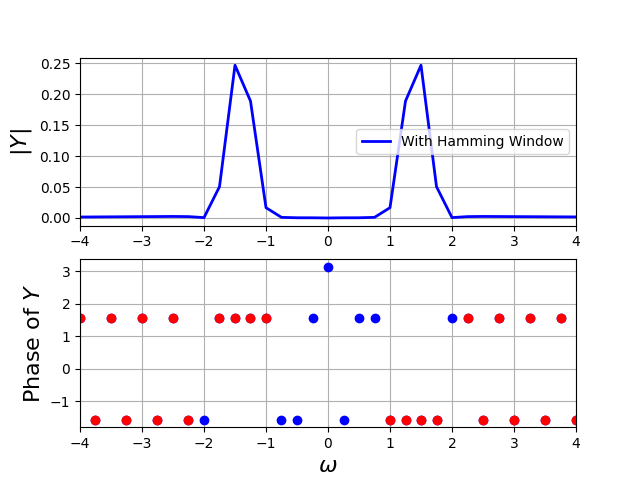
\includegraphics[scale=0.7]{fig1.png} 
    \caption{Spectrum of sin(\sqrt{2}t)}
    \label{fig:my_label}
\end{figure}

\subsection{cos$^3$(0.86t):}
Using the function \textbf{spectrum()}, we plot the DFT of cos$^3$(0.86t) with and without hamming window.
\lstinputlisting[language = python]{code2.py}
\begin{figure}[h!]

\begin{subfigure}{0.55\textwidth}
    \centering
    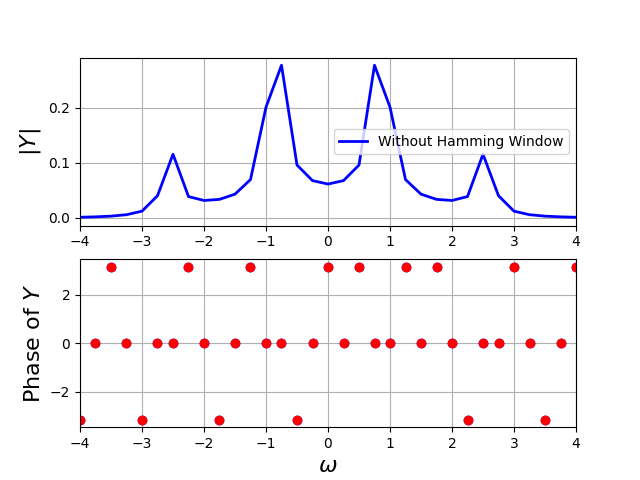
\includegraphics[scale=0.9,width=\linewidth]{fig2.png} 
    \caption{Without Hamming's Window}
    \label{fig:my_label}
\end{subfigure}
\begin{subfigure}{0.55\textwidth}
    \centering
    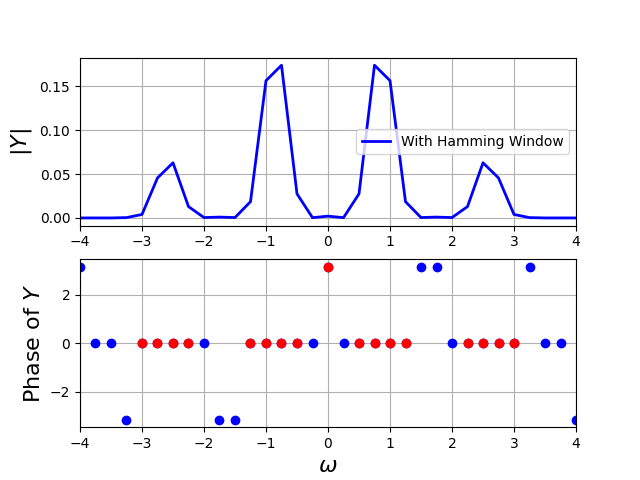
\includegraphics[scale=0.9,width=\linewidth]{fig3.png} 
    \caption{With Hamming's Window}
    \label{fig:image2}
\end{subfigure}


\end{figure}
\vspace{100mm}
\subsection{Estimating $\omega_o$ and $\delta$}
To find the estimate of $\omega_o$, we take the weighted average of $\omega$, with weights |Y($\omega$)|$^2$. For finding $\delta$, we use the lstsq() function. We form the matrices from the below equation,
For $\omega_o$ = 1.2 and $\delta$ = 1, the estimate we get is,
\begin{equation}
\omega_o = 1.1749137503896578
\end{equation}
\begin{equation}
    \delta = 1.0056655986981278
\end{equation}
The below code accomplishes the  above,
\noindent
\lstinputlisting[language = python]{code3.py}
\subsection{With the addition of Noise }
Undergoing the same process as before, the estimate of$\omega_o$ and $\delta$, with added Noise to the signals is,
\noindent
\begin{equation}
\omega_o = 1.0934953748562952
\end{equation}
\begin{equation}
    \delta = 0.9903572478888653
\end{equation}

\subsection{Chirped Signal}
The signal $cos(16(1.5+\frac{t}{2\pi})t)$ is given as input in 1024 steps. Using the \textbf{spectrum()} function, we plot the spectrum of the signal.
\noindent
\begin{figure}[h!]
    \centering
    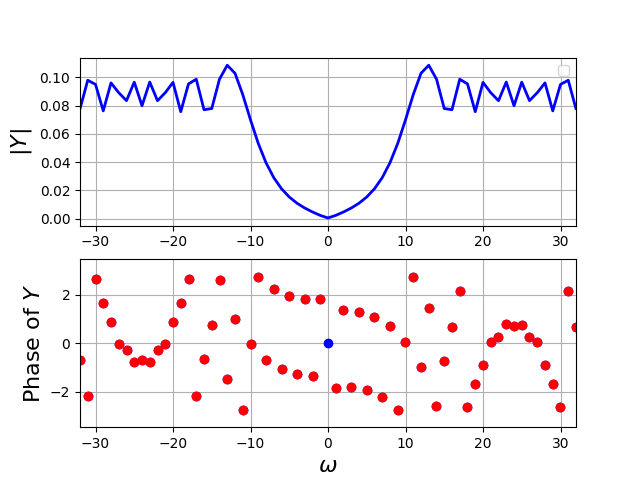
\includegraphics[scale=0.7]{fig4.png} 
    \caption{Spectrum of $cos(16(1.5+\frac{t}{2\pi})t)$}
    \label{fig:my_label}
\end{figure}
\subsection{Time-Frequency plot for the Chirped signal}
For the same chirped signal,  we break the 1024 vector into pieces that are 64 samples wide. Extract the DFT of each and store it as a column in a 2D array. Then plot the array as a surface plot to show how the signal's frequency varies with time. The below function accomplishes the above task.
\noindent
\lstinputlisting[language = python]{code4.py}
\begin{figure}[h!]
    \centering
    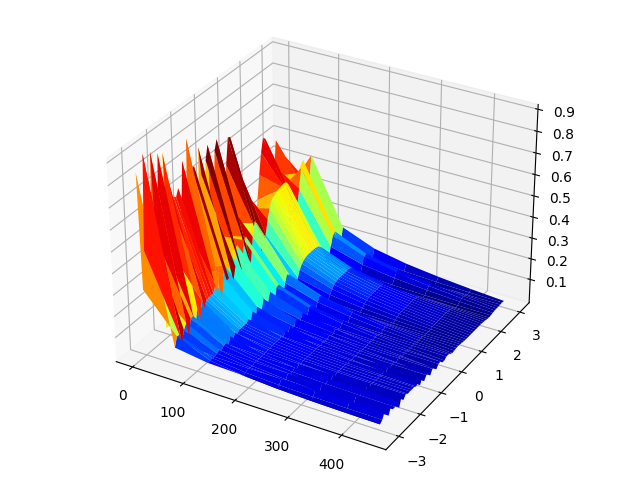
\includegraphics[scale=0.7]{fig5.png} 
    \caption{Time-Frequency Plot}
    \label{fig:my_label}
\end{figure}
\section{Conclusion}
DFTs of non-periodic signals can be computed in python with the help of a hamming window. Python


\end{document}

